\chapter{\MakeUppercase{Results and Discussion}}
\section{Aggregate Results}
Table \ref{tab:results_summary} summarizes the averaged simulation results. The values are taken from the generated result files in the \verb|plots| directory.

\begin{table}[h!]
	\centering
	\caption{Average simulation results across traffic levels}
	\renewcommand{\arraystretch}{1.25}
	\resizebox{\textwidth}{!}{
	\begin{tabular}{|l|l|c|c|c|c|c|}
		\hline
		\textbf{Protocol} & \textbf{Traffic} & \textbf{Delivery Ratio} & \textbf{Critical Delivery Ratio} & \textbf{Avg. Delay} & \textbf{Avg. Critical Delay} & \textbf{Overhead Ratio} \\
		\hline
		Epidemic & Low & 0.862 & 0.869 & 878.94 & 887.88 & 26.18 \\
		Epidemic & Medium & 0.851 & 0.814 & 983.63 & 981.18 & 26.61 \\
		Epidemic & High & 0.366 & 0.219 & 1829.59 & 1824.28 & 32.86 \\
		\hline
		Spray and Wait & Low & 0.764 & 0.768 & 1196.41 & 1192.24 & 8.43 \\
		Spray and Wait & Medium & 0.752 & 0.743 & 1157.54 & 1181.98 & 8.46 \\
		Spray and Wait & High & 0.682 & 0.577 & 1381.25 & 1375.01 & 8.87 \\
		\hline
		Spatio-Semantic & Low & 0.866 & 0.871 & 916.24 & 925.13 & 26.54 \\
		Spatio-Semantic & Medium & 0.860 & 0.828 & 945.70 & 925.65 & 25.61 \\
		Spatio-Semantic & High & 0.734 & 0.582 & 1377.54 & 1121.35 & 19.94 \\
		\hline
	\end{tabular}}
	\label{tab:results_summary}
\end{table}

\begin{table}[h!]
	\centering
	\caption{Buffer drops across traffic levels}
	\renewcommand{\arraystretch}{1.25}
	\begin{tabular}{|l|c|c|c|}
		\hline
		\textbf{Protocol} & \textbf{Low} & \textbf{Medium} & \textbf{High} \\
		\hline
		Epidemic & 0.00 & 39.50 & 828.40 \\
		\hline
		Spray and Wait & 0.00 & 1.45 & 316.80 \\
		\hline
		Spatio-Semantic & 0.00 & 31.50 & 588.55 \\
		\hline
	\end{tabular}
	\label{tab:buffer_drops}
\end{table}

\section{Delivery Ratio Analysis}
Figure \ref{fig:delivery_ratio} summarizes how overall delivery changes as traffic increases.

\begin{figure}[h!]
    \centering
    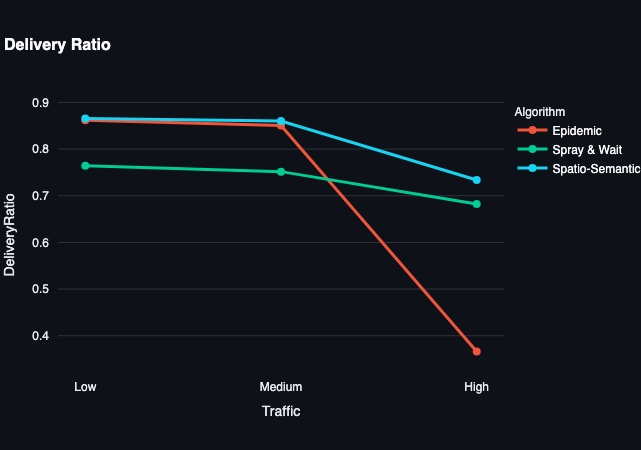
\includegraphics[width=0.85\textwidth]{images/delivery-ratio}
    \caption{Overall message delivery success ratio}
    \label{fig:delivery_ratio}
\end{figure}

At low traffic, Spatio-Semantic routing achieves a delivery ratio of 0.866, slightly above Epidemic routing at 0.862 and clearly above Spray and Wait at 0.764. This shows that the proposed utility rules do not harm reachability under light load.

At medium traffic, Spatio-Semantic routing reaches 0.860, compared with 0.851 for Epidemic routing and 0.752 for Spray and Wait. The gain over Spray and Wait is important because it shows that utility-guided forwarding can recover delivery opportunities lost by conservative copy-limited routing.

At high traffic, Epidemic routing collapses to 0.366 due to buffer pressure and excessive replication. Spray and Wait remains more stable at 0.682 because it controls copies. Spatio-Semantic routing achieves 0.734, which is 100.3 percent higher than Epidemic routing and 7.5 percent higher than Spray and Wait. This is the strongest evidence that the proposed protocol is better suited to congested disaster \acp{dtn}.

\section{Scenario-Wise Interpretation}
The low-traffic scenario is useful mainly as a sanity check. Under light load, most protocols have enough resources to perform reasonably well, so the main question is whether the proposed router introduces unnecessary complexity or harmful selectivity. The answer appears to be no. Spatio-Semantic routing remains competitive with Epidemic and clearly stronger than Spray and Wait, which means that the added utility logic does not reduce basic reachability.

The medium-traffic scenario reveals the beginning of congestion effects. Here, forwarding decisions start to matter more because not every copy can be replicated freely without consequence. The proposed router performs well in this regime because it still has enough opportunity to exploit spatial and semantic hints before buffers become severely stressed. Medium traffic is therefore an important transition point: it shows that the protocol does not only succeed at the extremes of either very easy or very difficult conditions.

The high-traffic scenario is the most informative because it resembles the stressed conditions that motivate the thesis. In this regime, the results separate the protocols clearly. Epidemic routing suffers from uncontrolled replication, and Spray and Wait preserves resources but becomes slower and more passive. Spatio-Semantic routing occupies the middle ground envisioned in the design chapter. It uses more transmissions than Spray and Wait, but those transmissions are directed by utility and priority rather than by blind flooding.

\section{Critical Delivery Analysis}
Figure \ref{fig:critical_delivery_ratio} focuses specifically on urgent traffic, which is the central concern of the thesis.

\begin{figure}[h!]
    \centering
    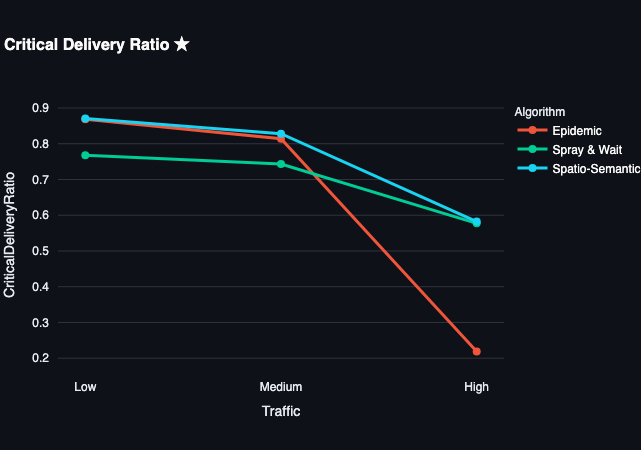
\includegraphics[width=0.85\textwidth]{images/critical-delivery-ratio}
    \caption{Delivery ratio specifically for high-priority critical messages}
    \label{fig:critical_delivery_ratio}
\end{figure}

Critical delivery ratio is the most important metric for the thesis objective. Under high traffic, Epidemic routing delivers only 0.219 of critical messages, while Spray and Wait delivers 0.577 and Spatio-Semantic delivers 0.582. The proposed protocol improves critical delivery by 166.2 percent over Epidemic routing. It is only slightly above Spray and Wait in ratio, but this ratio must be interpreted together with critical delay.

At medium traffic, Spatio-Semantic routing also performs best with a critical delivery ratio of 0.828 compared with 0.814 for Epidemic and 0.743 for Spray and Wait. The result indicates that the critical buffer reserve and priority-first forwarding help before the network reaches full congestion.

\section{Delay Analysis}
Figure \ref{fig:avg_critical_delay} shows the clearest timing advantage of the proposed protocol.

\begin{figure}[h!]
    \centering
    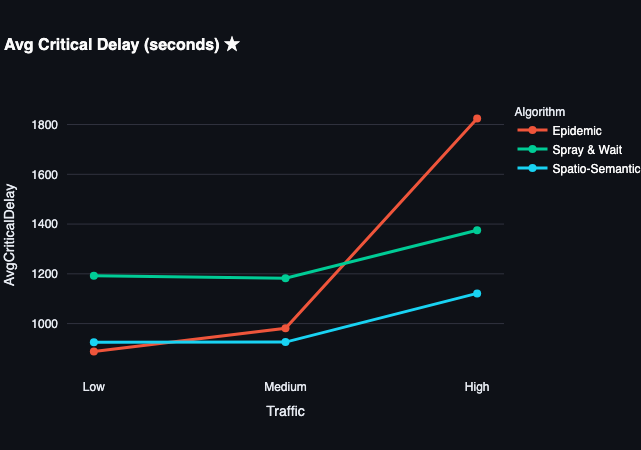
\includegraphics[width=0.85\textwidth]{images/avg-critical-delay.png}
    \caption{Average delivery delay for critical messages}
    \label{fig:avg_critical_delay}
\end{figure}

Delay is where the proposed protocol shows a major advantage over Spray and Wait. At high traffic, Spatio-Semantic routing reduces average critical delay to 1121.35 seconds. Epidemic routing requires 1824.28 seconds, and Spray and Wait requires 1375.01 seconds. Therefore, Spatio-Semantic routing reduces critical delay by 38.5 percent over Epidemic routing and 18.4 percent over Spray and Wait.

This result is consistent with the protocol design. Spray and Wait conserves transmissions but often waits for direct delivery after copies become scarce. Spatio-Semantic routing continues to hand off messages to better carriers based on spatial, semantic, and encounter utility. Critical messages therefore move toward useful relays instead of remaining with weak carriers.

\begin{figure}[h!]
    \centering
    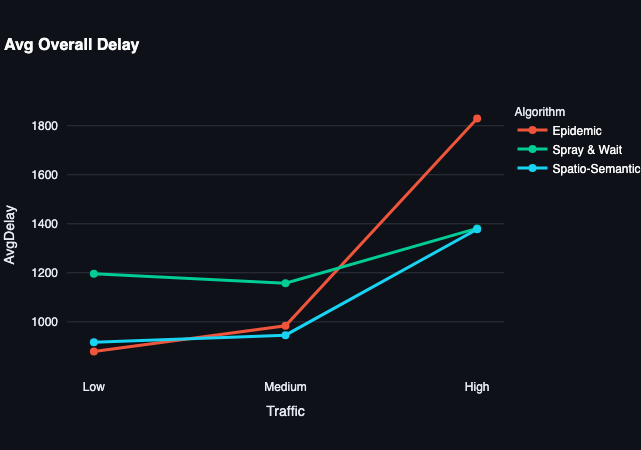
\includegraphics[width=0.85\textwidth]{images/avg-overall-delay}
    \caption{Average delivery delay for all messages}
    \label{fig:avg_overall_delay}
\end{figure}

Figure \ref{fig:avg_overall_delay} shows that the same pattern largely holds for all traffic, not only for critical messages. Epidemic is slightly faster under low load because flooding creates many early copies, but its delay rises sharply once congestion appears. Spatio-Semantic becomes the best or near-best protocol from medium traffic onward and slightly outperforms Spray and Wait even in the high-traffic case. This indicates that the proposed utility logic improves urgency handling without sacrificing overall timeliness.

\section{Interaction Between Metrics}
The metrics should not be interpreted in isolation. A protocol with high delivery but extreme delay may still be unsuitable for emergency communication. Likewise, a protocol with very low overhead may simply be failing to exploit available contacts. The proposed router is strongest when the metrics are read together: it preserves high delivery, maintains the best critical delay under high load, and reduces the worst congestion effects seen in Epidemic routing.

The relationship between critical delivery ratio and average critical delay is particularly important. Under high traffic, Spray and Wait and Spatio-Semantic achieve similar critical delivery ratios, but Spatio-Semantic delivers those critical messages substantially earlier. This distinction matters in practice because a disaster-response message that arrives much later may lose much of its operational value even if it is eventually counted as delivered. The proposed protocol therefore offers not only more reliable urgent delivery than flooding, but also more useful urgent delivery than passive waiting.

\begin{figure}[h!]
    \centering
    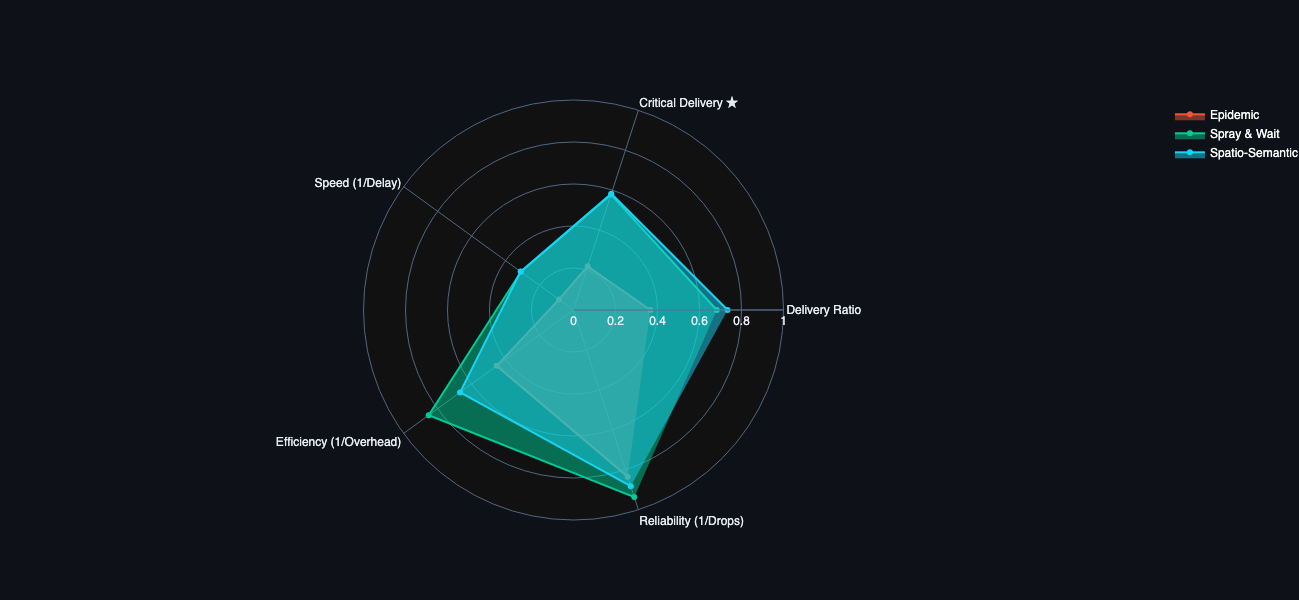
\includegraphics[width=0.85\textwidth]{images/performance-radar-high.png}
    \caption{Radar comparison of multi-objective routing performance}
    \label{fig:performance-radar-high-traffic}
\end{figure}

The high-traffic radar view in Figure \ref{fig:performance-radar-high-traffic} helps summarize this trade-off visually. It does not replace the numerical tables, but it makes the balance between delivery, urgency, overhead, and congestion easier to read in one place.

\section{Overhead and Drop Analysis}
\begin{figure}[h!]
    \centering
    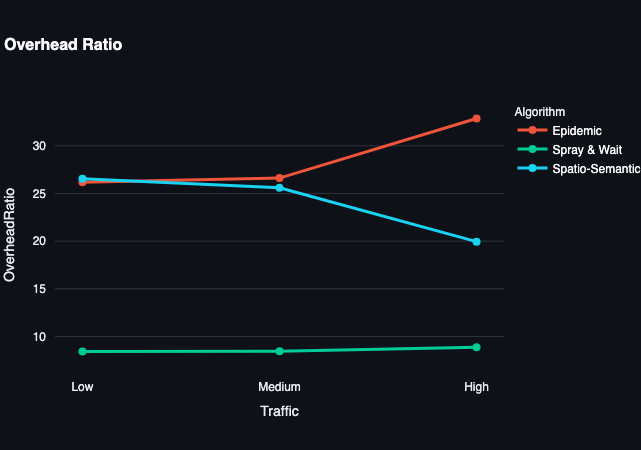
\includegraphics[width=0.85\textwidth]{images/overhead-ratio}
    \caption{Routing overhead ratio (transmissions per delivery)}
    \label{fig:overhead_ratio}
\end{figure}

The proposed protocol does not have the lowest overhead. Spray and Wait has the lowest overhead in all traffic levels because it is highly conservative. Under high traffic, Spray and Wait has an overhead ratio of 8.87, while Spatio-Semantic has 19.94. This is the main trade-off of the proposed design.

However, Spatio-Semantic routing is still more efficient than Epidemic routing under high traffic. Epidemic reaches an overhead ratio of 32.86 and 828.40 buffer drops. Spatio-Semantic reduces overhead by 39.3 percent and drops by 29.0 percent compared with Epidemic routing. The protocol therefore avoids the worst flooding behavior while preserving better delivery and delay than the conservative baseline.

\begin{figure}[h!]
    \centering
    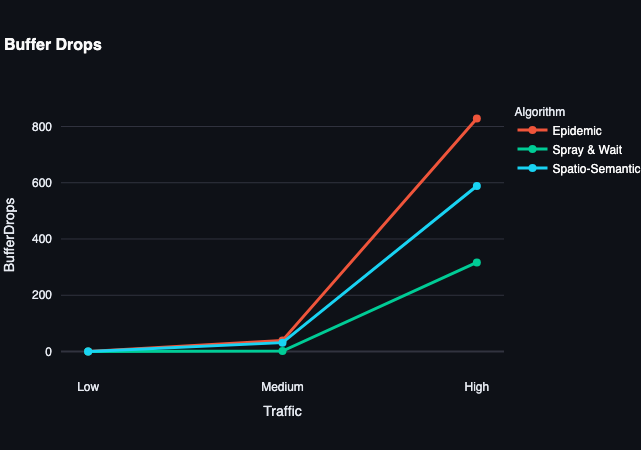
\includegraphics[width=0.85\textwidth]{images/buffer-drops}
    \caption{Comparison of buffer drops across traffic levels}
    \label{fig:buffer_drops}
\end{figure}

Figure \ref{fig:buffer_drops} shows the same congestion story from the storage side. Epidemic suffers the most severe collapse under heavy load, Spray and Wait protects buffers best, and Spatio-Semantic stays in between. That middle position is consistent with the design goal: spend more resources than Spray and Wait when the extra forwarding is useful, but avoid the uncontrolled replication that makes Epidemic fail under stress.

\section{Overall Discussion}
The results show that Spatio-Semantic routing is better than the compared protocols when the application values emergency delivery under stress. Epidemic routing is competitive only in low or moderate load but collapses under high traffic. Spray and Wait is efficient but slower and less adaptive. Spatio-Semantic routing uses additional transmissions purposefully: it favors drones, responders, nodes that visit destination zones, nodes with useful encounter histories, and critical-message preservation.

The most defensible conclusion is not that Spatio-Semantic routing is always the cheapest protocol. It is not. The correct conclusion is that it provides a stronger disaster-response trade-off: higher delivery than both baselines under high traffic, much better critical delay than both baselines under high traffic, and much better congestion behavior than Epidemic routing.

\section{Limitations of the Results}
The discussion should also acknowledge what the results do not prove. They do not show that the exact utility weights used in the protocol are globally optimal, nor do they show that the same gains will appear unchanged under every mobility model. The results support the usefulness of the combined spatial-semantic design within the defined simulator settings.

They also do not imply that overhead is unimportant. In very resource-constrained devices, the additional forwarding cost relative to Spray and Wait may require further tuning. However, the thesis context is disaster communication, where the operational cost of losing urgent messages can be greater than the cost of additional controlled transmissions. Within that application context, the measured trade-off remains favorable to the proposed protocol.

\section{Implications for Disaster Routing Design}
The findings have a broader implication for the design of disaster \ac{dtn} protocols. They suggest that relay selection should be guided by a richer notion of usefulness than simple replication count or raw encounter frequency alone. In disrupted environments, the most helpful carrier is often the one that combines mobility opportunity, role relevance, and current network context. The proposed protocol performs well because it encodes that broader notion in a practical way.

The results also support the idea that critical-traffic awareness should be built into congestion management itself. When buffers become pressured, message priority cannot remain a passive label. It must influence storage and forwarding decisions directly. The stronger high-traffic critical-delay results of the proposed protocol indicate that this integration is not only conceptually appealing but also measurably beneficial within the simulation setting used in the thesis.
